\newpage
\section{Functionalități}

În acest capitol sunt prezentate funcționalitățile implementate in aplicația dezvoltată. Aplicația afișează o diagrama 
care are la baza un model 3D format din mai multe elemente, punând accentul pe relațiile de legătura dintre elemente.\newline

Functionalități de bază:
\begin{itemize}
    \item încărcarea oricarui fișier .mdef și crearea diagramei
    \item modificarea diagramei create
    \begin{itemize}
        \item mutarea elementelor
        \item scalarea intregii diagrame
        \item schimbarea culorii anumitor elemente
    \end{itemize} 
    \item salvarea modificărilor într-un fisier separat
    \item încărcarea automata a fișierului salvat, dacă există
    \item afisarea modelului din mai multe perspective ortografice
    \item afisarea modelului sub formă de graf
    \item căutarea unui element dupa un cuvânt cheie și evidențierea lui
    \item compararea dintre diferite versiuni de modele
    \item afișarea unui panou de tip legendă care prezintă diferitele tipuri de elemente
    \item afișarea unui panou de informații în care sunt afișate informații adiționale legate de elementele selectate
\end{itemize}

În continuare sunt prezentate caracteristicile aplicației în detaliu. Pentru demonstrarea funcționalităților am folosit un fișier .mdef
pe baza modelului urmator.

\subsection{Încarcarea fișierelor}
Se pot încărca oricâte fișiere .mdef în aplicație, fiecare fișier fiind deschis într-un tab diferit. 
Acest lucru se face din meniul \verb|File| de unde se alege optiunea \verb|Open|, care v-a deschide o noua fereastra de 
unde utilizatorul își poate alege fișierul. 
Odată ales un fișier el este deschis într-un tab nou care conține o scena cu mai multe elemente de tip Motion body, 
Joint sau Connector.\newline

\begin{figure}[h]
    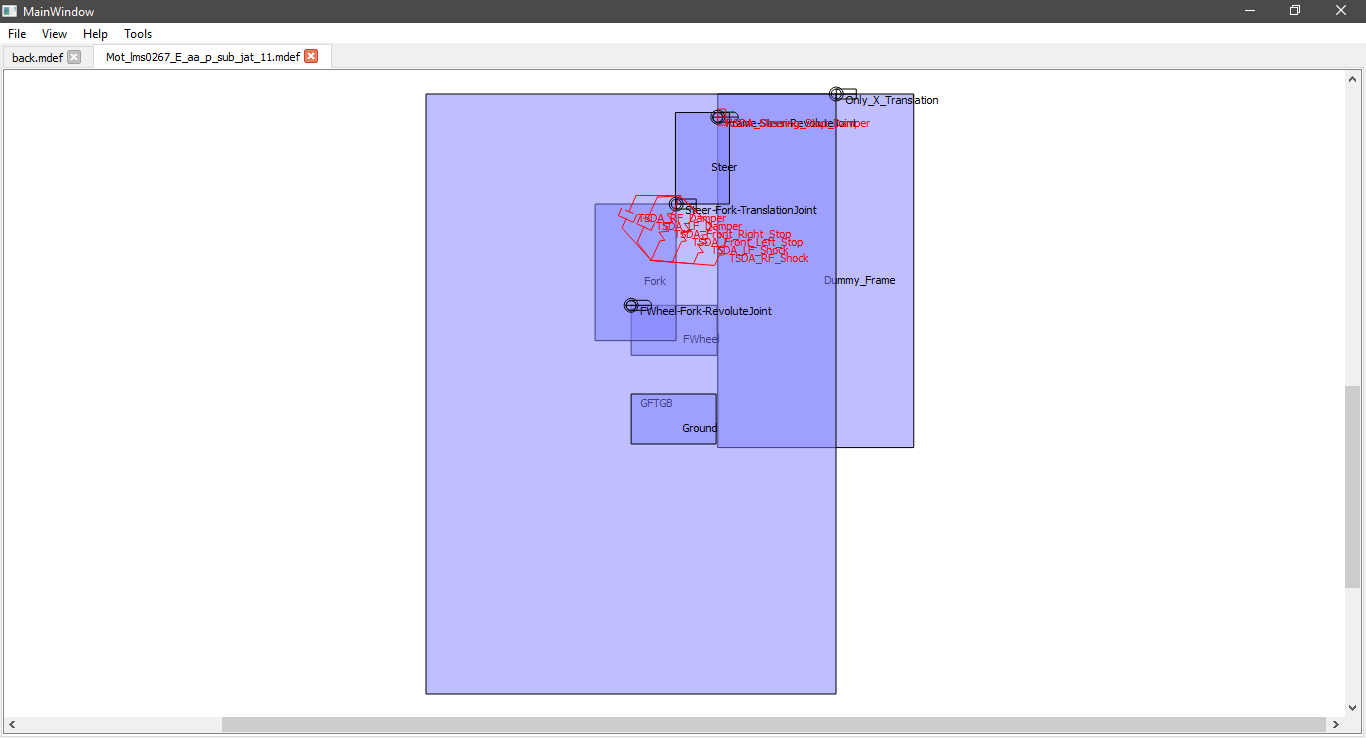
\includegraphics[width=\linewidth]{imagini/implementare/tabs.png}
    \caption{Un model deschis in aplicație}
    \label{fig:tabs}
\end{figure}

\subsection{Modificarea diagramei}
Diagrama creată se poate modifca prin:
\begin{itemize}
    \item schimbarea perspectivei ortografice
    \item afișarea sub forma de graf
    \item scalare
    \item modificarea pozițiilor elementelor
    \item modificarea culorii elementelor
\end{itemize}

Una dintre problemele întâmpinate în procesul de dezvolatere a aplicației a fost suprapunerea elementelor în anumite perspective. 
Această problemă a fost rezolvată prin două metode: prin scalare, care păstreaza pozițiile relative ale elemntelor în model, și prin afișarea 
modelului sub forma unui graf, care nu ia în considerare aspecte legate de poziții sau forme.\newline

Scalarea este necesară pentru modele mari având scopul de a pune în evidenta detalii care s-ar observa greu dacă întregul model este afisat în fereastră. 
Totodată pentru modul de afișare sub forma unei perspective ortografice, scalarea este utilă
pentru modelele în care se suprapun elemente. In acel mod prin scalare se scalează doar punctele de conectare ale legaturilor cu corpurile in schimb ce marimea 
corpurilor ramâne la fel.\newline

Mutarea elementelor poate fi utilă în cazul în care utilizatorul vrea sa organizeze în alt fel reprezentarea fișierul, sau daca există
anumite suprapuneri între elemente.\newline 

\begin{figure}[H]
    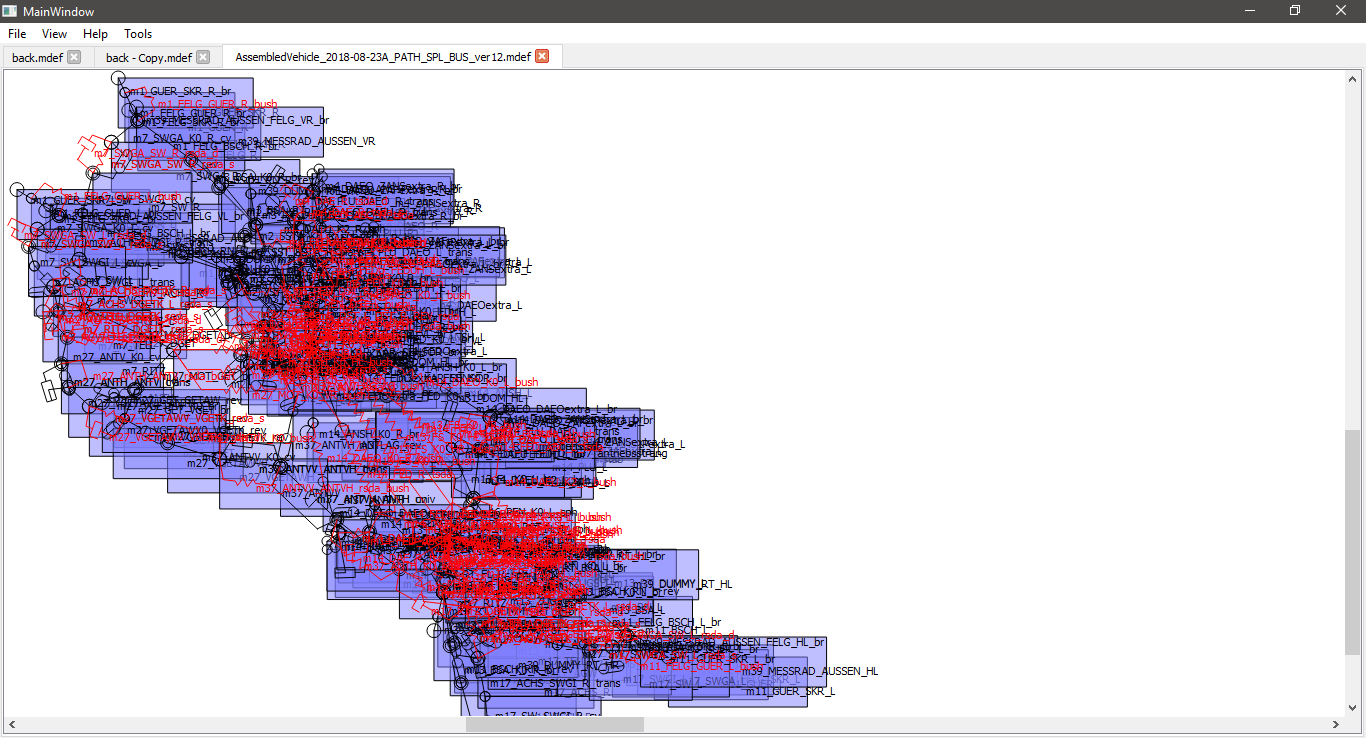
\includegraphics[width=\linewidth]{imagini/implementare/bigmodel.png}
    \caption{Un model cu multe elemente}
    \label{fig:tabs}

    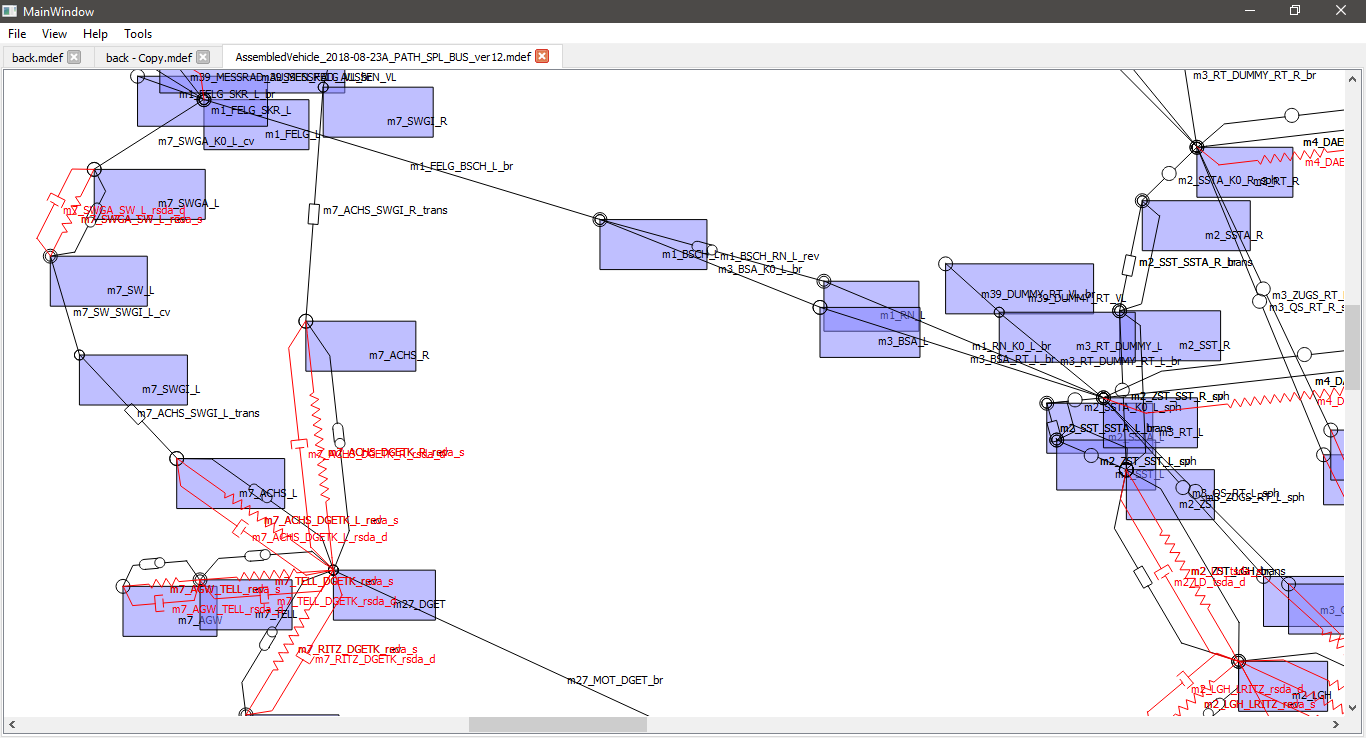
\includegraphics[width=\linewidth]{imagini/implementare/bigmodelzoom.png}
    \caption{Un model cu multe elemente}
    \label{fig:tabs}
\end{figure}

\subsection{Salvarea scenei modificate}
Toate schimbările legate de scena în care se afla toate elementele pot fi salvate într-un fișier XML separat. 
Dacă un model are salvată o scenă, ea este încărcată automat la deschiderea modelului.
Pentru salvarea automata se alege optinuea \verb|Save| din meniul \verb|File|, fisierul salvat se v-a afla într-un folder specific și v-a avea acelasi nume cu modelul.
Dacă se dorește ca modelul să fie salvat explicit într-un loc anume cu un nume diferit se poate alege \verb|Save as|. La fel dacă se dorește 
încărcarea unui fișier salvat anume, se elege opțiunea Load file.

\subsection{Afisarea sub forma unei perspective ortografice}
Fișierul reprezentând un model 3D, pentru a afișa structura de baza și relațiile dintre elemente în sine într-un plan 2D am 
ales folosirea noțiunii de perspectiva ortografica. Modelul este desenat în 2D, avand la bază coordonatele modelului
3D din fisierul .mdef, pentru fiecare perspectivă folosindu-se doua dintre cele trei coordonate, eliminănd una dintre ele. 
Astfel se obțin trei perspective individuale pentru afișarea modelului:

\begin{itemize}
    \item perspectiva laterala (side)
    \item perspectiva frontala (front)
    \item perspectiva de deasupra (top)
\end{itemize} 

Când un model este încărcat el este deschis automat in perspectiva laterală.
Formele elementelor din această opțiune au la bază coordonate reale citite din fișier. De exemplu mărimea dreptunghiului 
care reprezinta un Motionbody este calculată în funcție de pozițiile conexiunilor cu alte elemente și centrul de 
greutate. Aceste perspective pot fi alese de utilizator selectănd \verb|Perspective| din meniul \verb|View|. \newline

Această abordare este folositoare, din perspectiva utilizatorului, doar pentru modele cu un număr mic spre mediu de elemente 
deoarece pentru modele mai mari s-a observat că datorită structurii lor, în multe cazuri existau suprapuneri în oricare dintre 
cele trei perspective, făcând înțelegerea modelului mult mai grea.\newline 

\begin{figure}[h]
    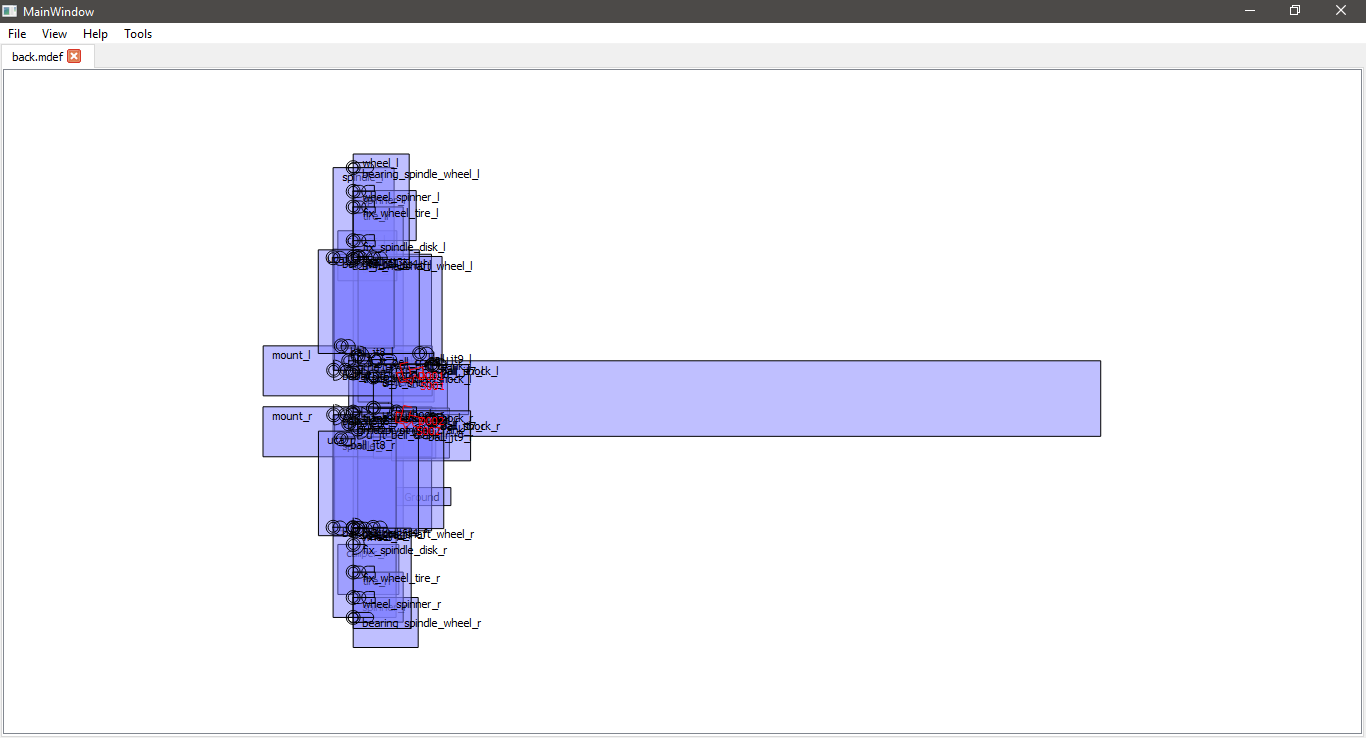
\includegraphics[width=\linewidth]{imagini/implementare/overlapping.png}
    \caption{Un model cu multe suprapuneri între elemente}
    \label{fig:tabs}
\end{figure}

\subsection{Afișarea sub forma de graf}
Pentru cazuri în care apar multe suprapuneri s-a implementat o structura de graf pentru reprezentarea modelului. 
In comparație cu perspectiva ortografică nu se ține cont de date precum puncte de conexiune sau centru de greutate și se bazează 
strict pe relațiile dintre elemente. Folosind un algoritm force-directed de desenare a unui graf obținem o structura mult mai organizata 
și mai inteligibilă, însa renunțam la concepte legate de forma modelului sau pozițiile elementelor în model.\newline

Această funcționalitate a fost adăugată având în gând un concept prezent în algoritmii force-directed și anume cel care garantează ca dacă un graf este planar, desenarea 
lui nu va conține suprapuneri intre muchii, și cel mai important, intre noduri. Totodata și pentru grafuri care nu sunt planare desenarea 
lui conține un număr minim de suprapuneri între muchii, de multe ori neglijabil, fiind în continuare ușor de înțeles.\newline

Opțiunea de graf poate fi aleasă alegând Force-directed din meniul \verb|View|. În această perspectivă se pot evidenția și tipurile de elemente Joint mai bine deoarece nu mai 
sunt reprezentate ca un punct fix dintre doua elemente Motion body ci dintr-o muchie cu un simbol pentru tipul elementului. 
Totodată din meniul de view se poate alege dacă este necesară afișarea fiecărui nume ale elementelor, acest lucru se face din meniul \verb|View| alegând \verb|Show names|, 
de unde se poate deselecta cate o căsuță pentru fiecare tip de element.\newline 

\begin{figure}[H]
    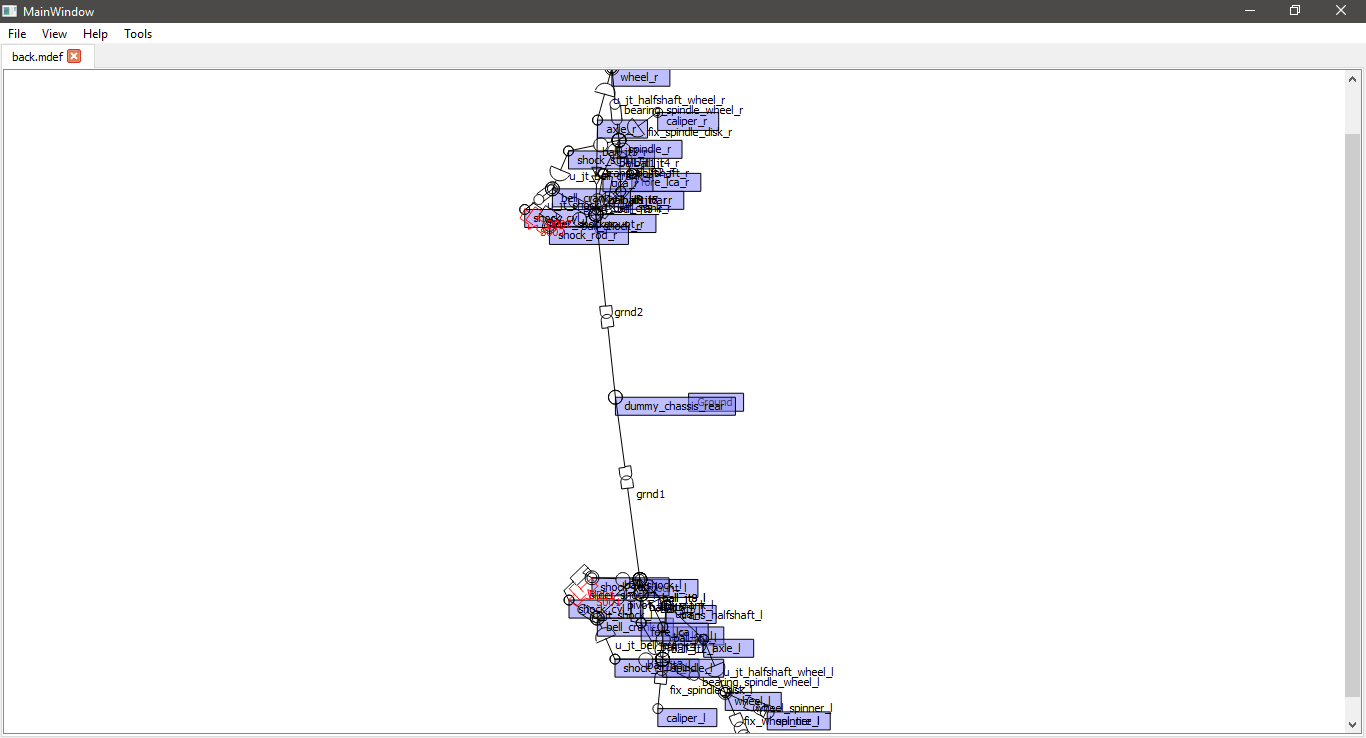
\includegraphics[width=\linewidth]{imagini/implementare/graf.png}
    \caption{Un model deschis in aplicație sub forma de graf}
    \label{fig:tabs}
\end{figure}

\subsection{Căutarea elementelor}
În continuare, pentru înțelegerea mai buna a modelului au fost implementate niște funcționalități de ajutor. 
O funcție de căutare pune în evidență anumite elemente din model. Se poate accesa din meniul \verb|Tools| de unde este deschisa o nouă fereastră cu mai multe opțiuni de cautare. 
Căutarea după un sub-string al cuvântului cheie sau căutarea după întreg cuvântul. Este prezenta și o opțiune de regex prin care utilizatorul poate 
cauta elemente după un anumit șablon. Din aceeași fereastra se poate alege dacă vrem sa cautam doar după anumite tipuri 
de elemente, precum și culoarea de selectare. După ce apăsam search, dacă căutarea a avut succes elementele sunt evidențiate în scena cu o culoare aleasă.
Utilizatorul poate efectua mai multe căutari cu diferite culori, lucru folositor pentru organizarea elementelor. 

\begin{figure}[H]
    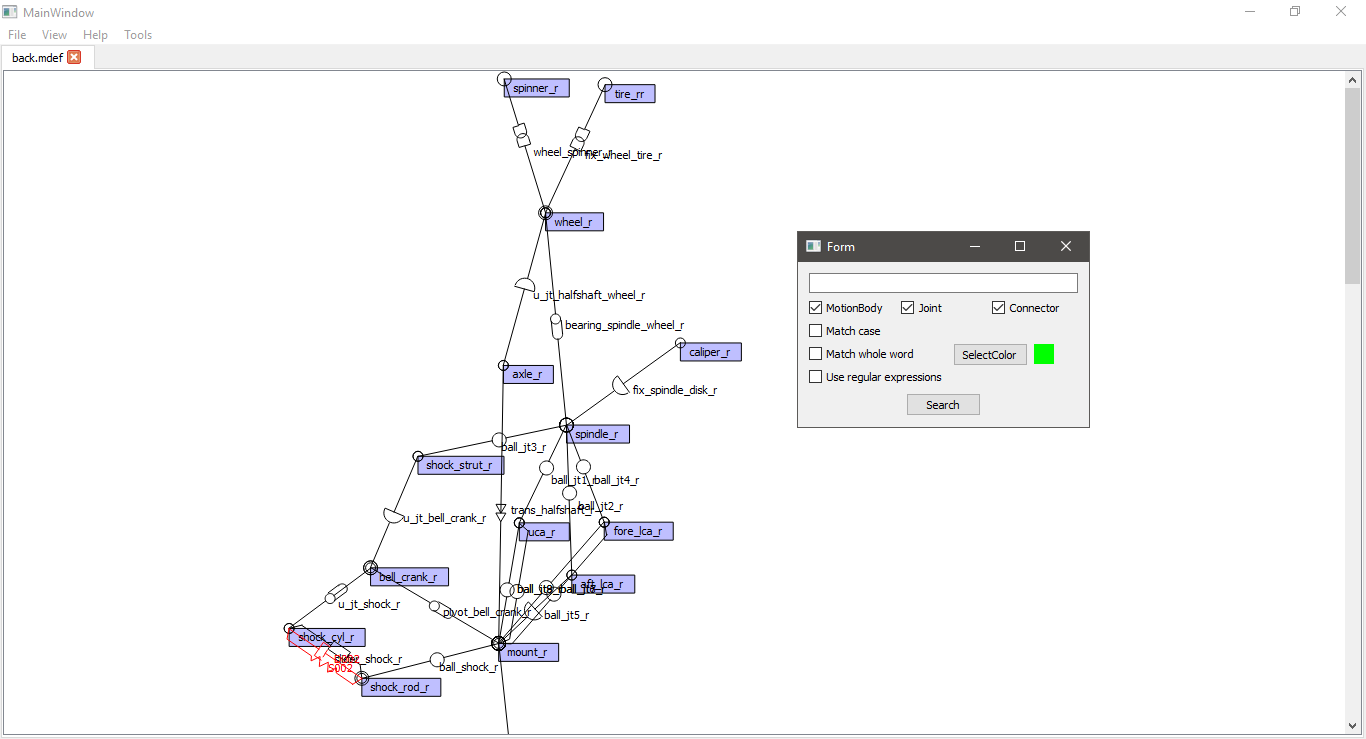
\includegraphics[width=\linewidth]{imagini/implementare/searchwindow.png}
    \caption{Fereastra de cautare}
    \label{fig:tabs}
\end{figure}

\subsection{Compararea modelelor}
Pentru evidențierea diferențelor dintre versiuni diferite de 
fișiere .mdef a fost implementată funcționalitatea \verb|Compare models|. Se poate accesa din meniul \verb|Tools|, opțiunea \verb|Compare models| și va deschide 
o nouă fereastră de unde utilizatorul poate alege ce modele vrea sa compare dintre cele deschise. Diferențe precum date diferite sunt evidențiate cu galben,
iar lipsa de elemente sunt evidențiate prin colorarea rosu, în modelul care conține elementul lipsă din modelul de comparare.\newline 

\begin{figure}[H]
    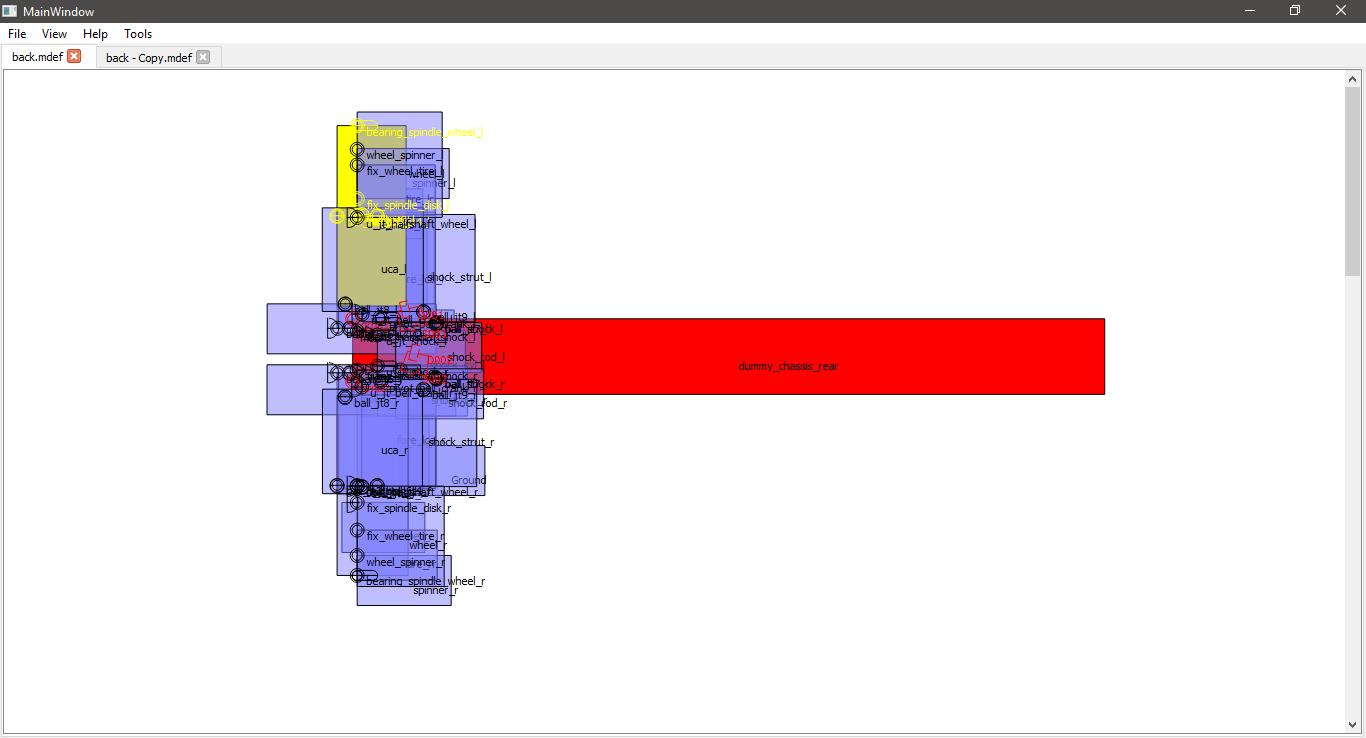
\includegraphics[width=\linewidth]{imagini/implementare/compare.png}
    \caption{Modelul principal comparat cu o alta versiune}
    \label{fig:tabs}
\end{figure}

\subsection{Informații adiționale}
O altă funcționalitate este cea a panoului de informații adiționale, acolo sunt afișate date din fișierul .mdef legate de un element 
anume. Aceste informații pot fi accesate prin click dreapta pe un element din scena. 
Date precum: 
\begin{itemize}
    \item tipul 
    \item originea
    \item relația cu alte elemente
\end{itemize}

\begin{figure}[H]
    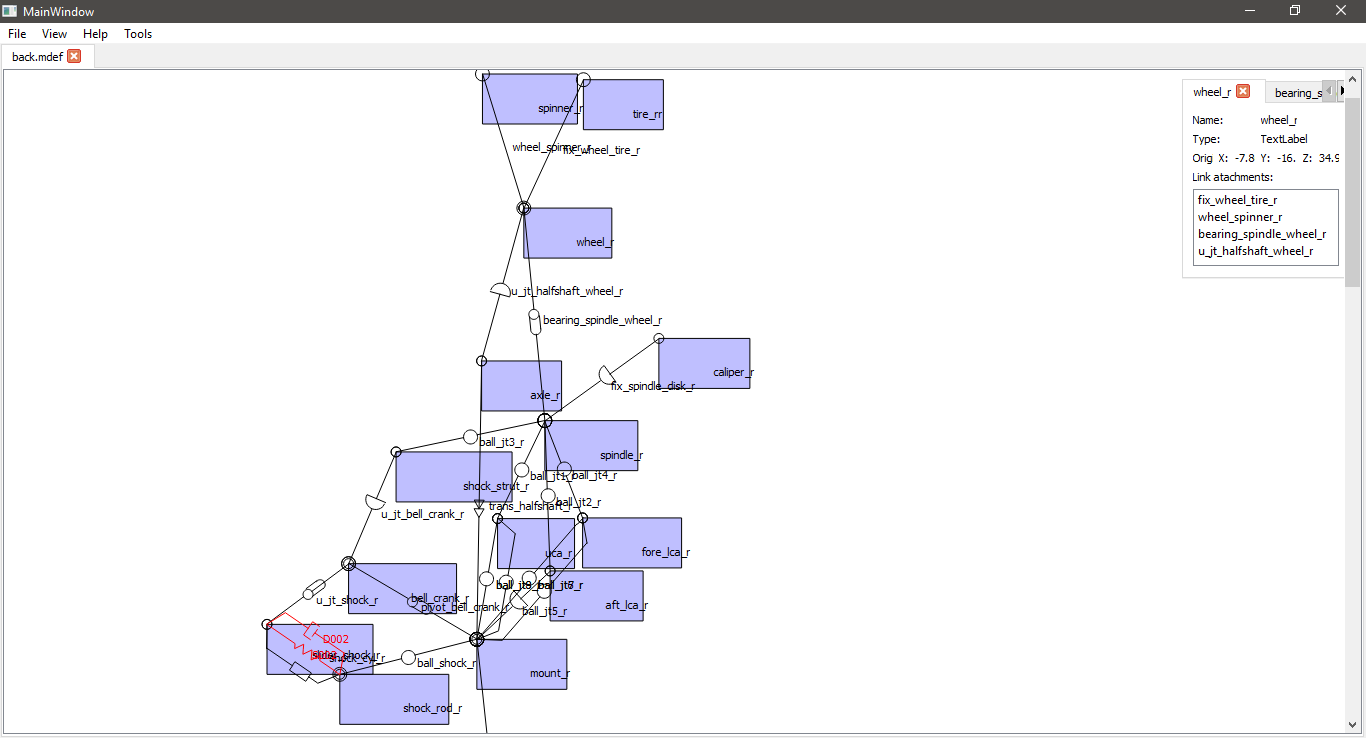
\includegraphics[width=\linewidth]{imagini/implementare/info.png}
    \caption{Panoul cu informatii despre un element Motion body}
    \label{fig:tabs}
\end{figure}

\subsection{Legenda}
O alta opțiune de ajutor este cea de legenda. 
Din \verb|help,legend| se deschide un nou panou care afișează toate simbolurile de elemente Joint și elemente Connectpr pentru ca 
utilizatorul sa înțeleagă mai bine structura modelului.\newline 

\begin{figure}[H]
    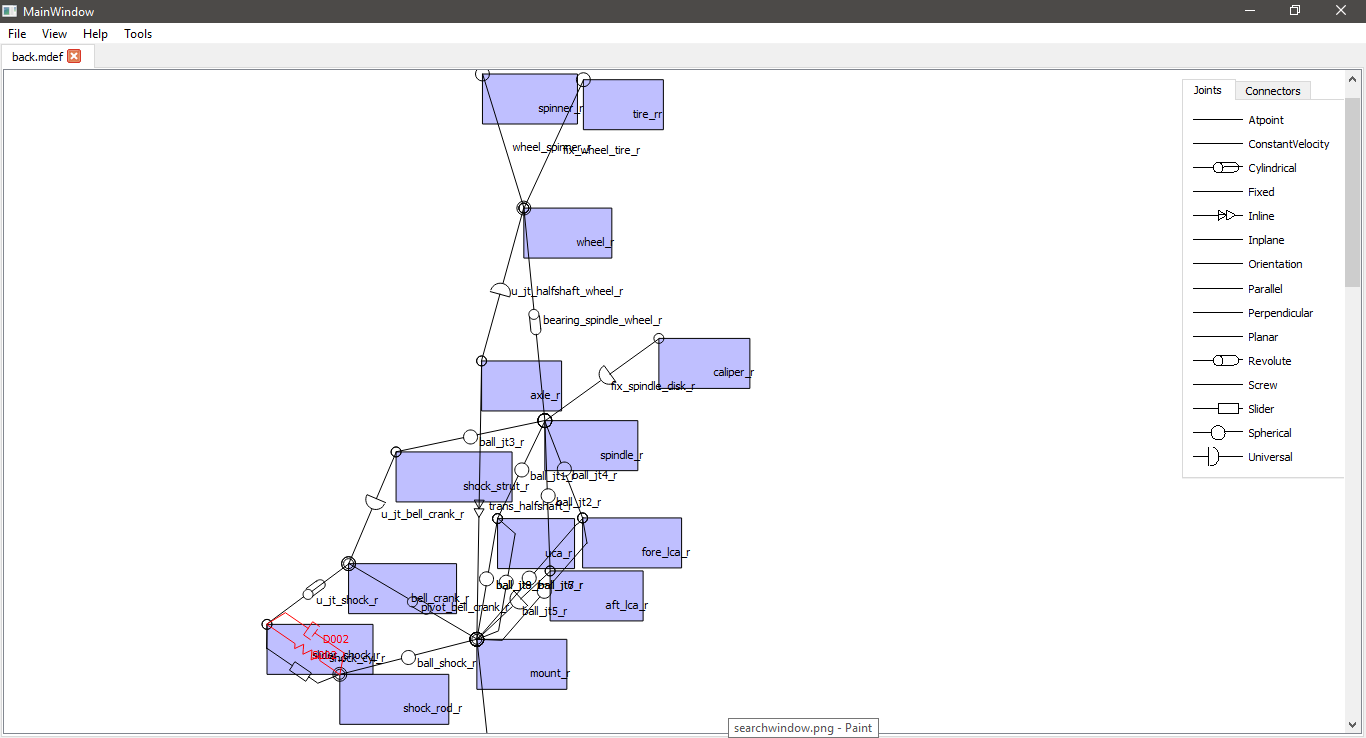
\includegraphics[width=\linewidth]{imagini/implementare/legend.png}
    \caption{Legenda}
    \label{fig:tabs}
\end{figure}
